\section{Equipment \& Software}

The CDI toolkit is a collection of demo code and examples to visualize
data from the Walabot sensor. It consists of a C++ wrapper
library/framework which makes it easy to implement new pieces of code
that uses the sensor data. The code uses opencv and vtk.

\subsection{Components of the toolkit}

\subsubsection{Sensor library}
this is a wrapper library around the C API provided as part of the
Walabot~\cite{walabot-spec} SDK. The library implements a framework
that provides interfaces and hooks for user code to implement. The
framework then calls into the user code with the appropriately
computed values.

\subsubsection{Demo}
Demo of webcam access that enlarges window as the user moves closer to
it and makes it smaller as they go closer.

\subsubsection{Tools}
There is a debugging tool that uses opencv to visualize signals coming
from the Walabot sensor.

\begin{figure}[H]
  \begin{center}
    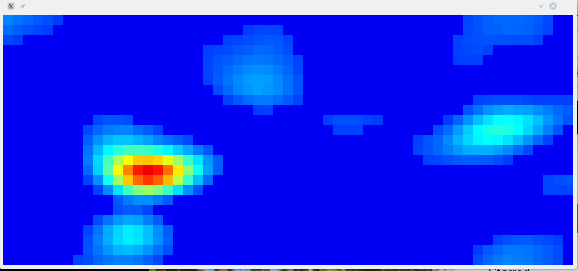
\includegraphics[scale=.85]{figures/visualization_debugging}
    \caption{Screenshot from the visualization debugging tool}
    \label{fig:debug_screenshot}
  \end{center}
\end{figure}

All the relevant code is located at \url{https://gitlab.com/hnaik/cdi/}

